
\section[{Characters, Glyphs, and Writing Modes}]{Characters, Glyphs, and Writing Modes}\label{WD}\par
Chapter \textit{\hyperref[CH]{vi\ Languages and Character Sets}} introduced the fundamental notions of language identification and character representation in an encoded TEI document. In this chapter we discuss some additional issues relating to the way that written language is represented in a TEI document. In sections \textit{\hyperref[WDNE]{5.1.\ Is Your Journey Really Necessary?}} and \textit{\hyperref[D25-20]{5.2.\ Markup Constructs for Representation of Characters and Glyphs}} we introduce markup which may be used to represent and document non-standard characters, that is, written symbols for which no codepoint exists in Unicode. The same markup may be used to annotate existing characters according to their visual or other properties, and thus process them as distinct glyphs (see section \textit{\hyperref[D25-30]{5.3.\ Annotating Characters}}), or to define new characters or glyphs (section \textit{\hyperref[D25-40]{5.4.\ Adding New Characters}}). We also provide recommendations concerning the Unicode Private Use Area (\textit{\hyperref[D25-50]{5.5.\ How to Use Code Points from the Private Use Area}}. Finally, in section \textit{\hyperref[WDWM]{5.6.\ Writing Modes}} we discuss ways of documenting the writing mode used in a source text, that is, the directionality of the script, the orientation of individual characters, and related questions.
\subsection[{Is Your Journey Really Necessary?}]{Is Your Journey Really Necessary?}\label{WDNE}\par
Despite the availability of Unicode, text encoders still sometimes find that the published repertoire of available characters is inadequate to their needs. This is particularly the case when dealing with ancient languages, for which encoding standards do not yet exist, or where an encoder wishes to represent variant forms of a character or \textit{glyphs}. The module defined by this chapter provides a mechanism to satisfy that need, while retaining compatibility with standards.\par
When encoders encounter some graphical unit in a document which is to be represented electronically, the first issue to be resolved should be ‘Is this really a different character?’ To determine whether a particular graphical unit \textit{is} a character or not, see \textit{\hyperref[D4-42]{vi.2.2\ Terminology and Key Concepts}}.\par
If the unit is indeed determined to be a character, the next question should be ‘Has this character been encoded already?’ In order to determine whether a character has been encoded, encoders should follow the following steps: \begin{enumerate}
\item \par
Check the Unicode web site at \url{http://www.unicode.org}, in particular the page \xref{http://unicode.org/standard/where/}{"Where is my Character?"}, and the associated character code charts. Alternatively, users can check the latest published version of \textit{The Unicode Standard} (\hyperref[CH-BIBL-3]{Unicode Consortium (2006)}), though the web site is often more up to date than the printed version, and should be checked for preference. \par
The pictures (‘glyphs’) in the Unicode code charts are only meant to be representative, not definitive. If a specific form of an already encoded character is required for a project, refer to the guidelines contained below under \hyperref[D25-30]{Annotating Characters}. Remember that your encoded document may be rendered on a system which has different fonts from yours: if the specific form of a character is important to you, then you should document it.
\item Check the Proposed New Characters web page (\url{http://unicode.org/alloc/Pipeline.html}) to see whether the character is in line for approval.
\item Ask on the Unicode email list (\url{http://www.unicode.org/consortium/distlist.html}) to see whether a proposal is pending, or to determine whether this character is considered eligible for addition to the Unicode Standard.
\end{enumerate}\par
Since there are now over 130,000 characters in Unicode, chances are good that what you need is already there, but it might not be easy to find, since it might have a different name in Unicode. Editors working with East Asian writing systems should consult the \xref{https://unicode.org/charts/unihan.html}{Unihan Database}. Look again, this time at other sites, preferably ones which also provide searches based on scripts and languages. For example \url{https://www.chise.org} (for CJK characters) or \url{http://www.eki.ee/letter/} (for non-CJK characters) . Take care, however, that all the properties of what seems to be a relevant character are consistent with those of the character you are looking for. For example, if your character is definitely a digit, but the properties of the best match you can find for it say that it is a letter, you may have a character not yet defined in Unicode.\par
In general, it is advisable to avoid Unicode characters generally described as presentation forms.\footnote{Specifically, characters in the Unicode blocks Alphabetic Presentation Forms, Arabic Presentation Forms-A, Arabic Presentation Forms-B, Letterlike Symbols,and Number Forms.} However, if the character you are looking for is being used in a notation (rather than as part of the orthography of a language) then it is quite acceptable to select characters from the Mathematical Operators block, provided that they have the appropriate properties (i.e. \texttt{So}: Symbol, Other; or \texttt{Sm}: Symbol, Math).\par
An encoded character may be precomposed or it may be formed from base characters and combining diacritical marks. Either will suffice for a character to be "found" as an encoded character. If there are several possible Unicode characters to choose amongst, it is good practice to consult other colleagues and practitioners to see whether a consensus has emerged in favour of one or other of them.\par
If, however, no suitable form of your character seems to exist, the next question will be: ‘Does the graphical unit in question represent a variant form of a known character, or does it represent a completely unencoded character?’ If the character is determined to be missing from the Unicode Standard, it would be helpful to submit the new character for inclusion (see \url{http://unicode.org/pending/proposals.html}). For assistance on writing or submitting a proposal, potential proposers can contact the UC Berkeley Script Encoding Initiative (\url{http://linguistics.berkeley.edu/sei/}).\par
These guidelines will help you proceed once you have identified a given graphical unit as either a variant or an unencoded character. Determining this will require knowledge of the contents of the document that you have. The first case will be called \textit{annotation} of a character, while the second case will be called \textit{adding} of a new character. How to handle graphical units that represent variants will be discussed below (\textit{\hyperref[D25-30]{5.3.\ Annotating Characters}}) while the problem of representing new characters will be dealt with in section \textit{\hyperref[D25-40]{5.4.\ Adding New Characters}}.\par
While there is some overlap between these requirements, distinct specialized markup constructs have been created for each of these cases. These constructs are presented in section \textit{\hyperref[D25-20]{5.2.\ Markup Constructs for Representation of Characters and Glyphs}} below.
\subsection[{Markup Constructs for Representation of Characters and Glyphs}]{Markup Constructs for Representation of Characters and Glyphs}\label{D25-20}\par
An XML document can, in principle, contain any defined Unicode character. The standard allows these characters to be represented either directly, using an appropriate encoding (UTF-8 by default), or indirectly by means of a \textit{numeric character reference} (NCR), such as \texttt{\&\#196;} (A-umlaut). The encoder can also restrict the range of characters which are represented directly in a document (or part of it) by adding a suitable encoding declaration. For example, if a document begins with the declaration \texttt{<?xml encoding="iso-8859-1"?>} any Unicode characters which are not in the ISO-8859-1 character set must be represented by NCRs.\par
The \textit{gaiji} module defined by this chapter adds a further way of representing specific characters and glyphs in a document. (Gaiji is from Japanese {\textJapanese 外字}, meaning  \textit{external characters}.) This allows the encoder to distinguish characters and glyphs which Unicode regards as identical, to add new nonstandard characters or glyphs, and to represent Unicode characters not available in the document encoding by an alternative means.\par
The mechanism provided here consists functionally of two parts: \begin{enumerate}
\item an element \hyperref[TEI.g]{<g>}, which serves as a proxy for new characters or glyphs
\item elements \hyperref[TEI.char]{<char>} and \hyperref[TEI.glyph]{<glyph>}, providing information about such characters or glyphs; these elements are stored in the \hyperref[TEI.charDecl]{<charDecl>} element in the header.
\end{enumerate}\par
When the gaiji module is included in a schema, the \hyperref[TEI.charDecl]{<charDecl>} element is added to the \textsf{model.encodingDescPart} class, and the \hyperref[TEI.g]{<g>} element is added to the phrase class. These elements and their components are documented in the rest of this section.\par
The Unicode standard defines properties for all the characters it defines in the \xref{https://unicode.org/ucd/}{Unicode Character Database}, knowledge of which is usually built into text processing systems. If the character represented by the \hyperref[TEI.g]{<g>} element does not exist in Unicode at all, its properties are not available. If the character represented is an existing Unicode character, but is not available in the document character set recognized by a given text processing system, it may also be convenient to have access to its properties in the same way. The \hyperref[TEI.char]{<char>} element makes it possible to store properties for use by such applications in a standard way.\par
The list of attributes (properties) for characters is modelled on those in the Unicode Character Database, which distinguishes \textit{normative} and \textit{informative} character properties. The Unicode Consortium also maintains a separate set of character properties specific to East Asian characters in the \xref{http://www.unicode.org/charts/unihan.html}{Unihan database} which TEI fully supports. Lastly, non-Unicode properties may also be supplied. Since the list of properties will vary with different versions of the Unicode Standard, there may not be an exact correspondence between them and the list of properties defined in these Guidelines.\par
Usage examples for these elements are given below at \textit{\hyperref[D25-30]{5.3.\ Annotating Characters}} and \textit{\hyperref[D25-40]{5.4.\ Adding New Characters}}. The gaiji module itself is formally defined in section \textit{\hyperref[WSD-DEF]{5.10.\ Formal Definition}} below. It declares the following additional elements: 
\begin{sansreflist}
  
\item [\textbf{<charDecl>}] (character declarations) provides information about nonstandard characters and glyphs.
\item [\textbf{<g>}] (character or glyph) represents a glyph, or a non-standard character.\hfil\\[-10pt]\begin{sansreflist}
    \item[@{\itshape ref}]
  points to a description of the character or glyph intended.
\end{sansreflist}  
\end{sansreflist}
 The \hyperref[TEI.charDecl]{<charDecl>} element is a member of the class \textsf{model.encodingDescPart}, and thus becomes available within \hyperref[TEI.encodingDesc]{<encodingDesc>} when this module is included in a schema. The \hyperref[TEI.g]{<g>} element is the only member of the class \textsf{model.gLike}: this class is referenced as an alternative to plain text in almost every element which contains plain text, thus permitting the \hyperref[TEI.g]{<g>} element also to appear at such places when this module is included in a schema.\par
The following elements may appear within a \hyperref[TEI.charDecl]{<charDecl>} element: 
\begin{sansreflist}
  
\item [\textbf{<desc>}] (description) contains a short description of the purpose, function, or use of its parent element, or when the parent is a documentation element, describes or defines the object being documented. 
\item [\textbf{<char>}] (character) provides descriptive information about a character.
\item [\textbf{<glyph>}] (character glyph) provides descriptive information about a character glyph.
\end{sansreflist}
\par
The \hyperref[TEI.char]{<char>} and \hyperref[TEI.glyph]{<glyph>} elements have similar contents and are used in similar ways, but their functions are different. The \hyperref[TEI.char]{<char>} element is provided to define a character which is not available in the current document character set, for whatever reason, as stated above. The \hyperref[TEI.glyph]{<glyph>} element is used to annotate a character that has already been defined somewhere (either in the document character set, or through a \hyperref[TEI.char]{<char>} element) by providing a specific glyph that shows how a character appeared in the original document. This is necessary since Unicode code points refer not to a single, specific glyph shape of a character, but rather to a set of glyphs, any of which may be used to render the code point in question; in some cases they can differ considerably.\par
The \hyperref[TEI.glyph]{<glyph>} element is provided for cases where the encoder wants to specify a specific glyph (or family of glyphs) out of all possible glyphs. Unfortunately, due to the way Unicode has been defined, there are cases where several glyphs that logically belong together have been given separate code points, especially in the blocks defining East Asian characters. In such cases, \hyperref[TEI.glyph]{<glyph>} elements can also be used to express the view that these apparently distinct characters are to be regarded as instances of the same character (see further \textit{\hyperref[D25-30]{5.3.\ Annotating Characters}}).\par
The Unicode Standard recommends naming conventions which should be followed strictly where the intention is to annotate an existing Unicode character, and which may also be used as a model when creating new names for characters or glyphs\footnote{It should be noted, however, that this naming convention cannot meaningfully be applied to East Asian characters; the typical Unicode descriptions for these characters take the form ‘CJK Unified Ideograph \texttt{U+4E00}’, where \texttt{U+4E00} is simply the Unicode code point value of the character in question. In cases where no Unicode code point exists, there is little hope of finding a name that helps to identify the character. Names should therefore be constructed in a way meaningful to local practice, for example by using a reference number from a well-known character dictionary or a project-specific serial number.}:\par
Within both \hyperref[TEI.char]{<char>} and \hyperref[TEI.glyph]{<glyph>}, the following elements are available: 
\begin{sansreflist}
  
\item [\textbf{<gloss>}] (gloss) identifies a phrase or word used to provide a gloss or definition for some other word or phrase.
\item [\textbf{<unicodeProp>}] (unicode property) provides a Unicode property for a character (or glyph).
\item [\textbf{<unihanProp>}] (unihan property) holds the name and value of a normative or informative Unihan character (or glyph) property as part of its attributes.
\item [\textbf{<localProp>}] (locally defined property) provides a locally defined character (or glyph) property.
\item [\textbf{<desc>}] (description) contains a short description of the purpose, function, or use of its parent element, or when the parent is a documentation element, describes or defines the object being documented. 
\item [\textbf{<mapping>}] (character mapping) contains one or more characters which are related to the parent character or glyph in some respect, as specified by the {\itshape type} attribute.
\item [\textbf{<figure>}] (figure) groups elements representing or containing graphic information such as an illustration, formula, or figure.
\item [\textbf{<note>}] (note) contains a note or annotation.
\end{sansreflist}
\par
Four of these elements (\hyperref[TEI.gloss]{<gloss>}, \hyperref[TEI.desc]{<desc>}, \hyperref[TEI.figure]{<figure>}, and \hyperref[TEI.note]{<note>}) are defined by other TEI modules, and their usage here is no different from their usage elsewhere. The \hyperref[TEI.figure]{<figure>} element, however, is used here only to link to an image of the character or glyph under discussion, or to contain a representation of it in SVG. The \hyperref[TEI.figure]{<figure>} element may contain more than one \hyperref[TEI.graphic]{<graphic>} element, for example to provide images with different resolution, or in different formats, or may itself be repeated. As elsewhere, the {\itshape mimeType} attribute of \hyperref[TEI.graphic]{<graphic>} should be used to specify the format of the image.\par
The \hyperref[TEI.mapping]{<mapping>} element is similar to the standard TEI \hyperref[TEI.equiv]{<equiv>} element. While the latter is used to express correspondence relationships between TEI concepts or elements and those in other systems or ontologies, the former is used to express any kind of relationship between the character or glyph under discussion and characters or glyphs defined elsewhere. It may contain any Unicode character, or a \hyperref[TEI.g]{<g>} element linked to some other \hyperref[TEI.char]{<char>} or \hyperref[TEI.glyph]{<glyph>} element, if, for example, the intention is to express an association between two non-standard characters. The type of association is indicated by the {\itshape type} attribute, which may take such values as \texttt{exact} for exact equivalences, \texttt{uppercase} for uppercase equivalences, \texttt{lowercase} for lowercase equivalences, \texttt{standard} for standardized forms, and \texttt{simplified} for simplified characters, etc., as in the following example: \par\bgroup\index{charDecl=<charDecl>|exampleindex}\index{char=<char>|exampleindex}\index{localProp=<localProp>|exampleindex}\index{name=@name!<localProp>|exampleindex}\index{value=@value!<localProp>|exampleindex}\index{localProp=<localProp>|exampleindex}\index{name=@name!<localProp>|exampleindex}\index{value=@value!<localProp>|exampleindex}\index{mapping=<mapping>|exampleindex}\index{type=@type!<mapping>|exampleindex}\exampleFont \begin{shaded}\noindent\mbox{}{<\textbf{charDecl}>}\mbox{}\newline 
\hspace*{1em}{<\textbf{char}\hspace*{1em}{xml:id}="{aenl}">}\mbox{}\newline 
\hspace*{1em}\hspace*{1em}{<\textbf{localProp}\hspace*{1em}{name}="{name}"\mbox{}\newline 
\hspace*{1em}\hspace*{1em}\hspace*{1em}{value}="{LATIN LETTER ENLARGED SMALL A}"/>}\mbox{}\newline 
\hspace*{1em}\hspace*{1em}{<\textbf{localProp}\hspace*{1em}{name}="{entity}"\hspace*{1em}{value}="{aenl}"/>}\mbox{}\newline 
\hspace*{1em}\hspace*{1em}{<\textbf{mapping}\hspace*{1em}{type}="{standard}">}a{</\textbf{mapping}>}\mbox{}\newline 
\hspace*{1em}{</\textbf{char}>}\mbox{}\newline 
{</\textbf{charDecl}>}\end{shaded}\egroup\par \par
The mapping element may also be used to represent a mapping of the character or (more likely) glyph under discussion onto a character from the private use area as in this example: \par\bgroup\index{charDecl=<charDecl>|exampleindex}\index{glyph=<glyph>|exampleindex}\index{localProp=<localProp>|exampleindex}\index{name=@name!<localProp>|exampleindex}\index{value=@value!<localProp>|exampleindex}\index{mapping=<mapping>|exampleindex}\index{type=@type!<mapping>|exampleindex}\index{mapping=<mapping>|exampleindex}\index{type=@type!<mapping>|exampleindex}\exampleFont \begin{shaded}\noindent\mbox{}{<\textbf{charDecl}>}\mbox{}\newline 
\hspace*{1em}{<\textbf{glyph}\hspace*{1em}{xml:id}="{z103}">}\mbox{}\newline 
\hspace*{1em}\hspace*{1em}{<\textbf{localProp}\hspace*{1em}{name}="{name}"\mbox{}\newline 
\hspace*{1em}\hspace*{1em}\hspace*{1em}{value}="{LATIN LETTER Z WITH TWO STROKES}"/>}\mbox{}\newline 
\hspace*{1em}\hspace*{1em}{<\textbf{mapping}\hspace*{1em}{type}="{standard}">}Z{</\textbf{mapping}>}\mbox{}\newline 
\hspace*{1em}\hspace*{1em}{<\textbf{mapping}\hspace*{1em}{type}="{PUA}">}U+E304{</\textbf{mapping}>}\mbox{}\newline 
\hspace*{1em}{</\textbf{glyph}>}\mbox{}\newline 
{</\textbf{charDecl}>}\end{shaded}\egroup\par \par
A more precise documentation of the properties of any character or glyph may be supplied using one of the three ‘property’ elements: \hyperref[TEI.localProp]{<localProp>}, \hyperref[TEI.unicodeProp]{<unicodeProp>}, or \hyperref[TEI.unihanProp]{<unihanProp>}; these are described in the next section.
\subsubsection[{Character Properties}]{Character Properties}\label{ucsprops}\par
The Unicode Standard documents ‘ideal’ characters, defined by reference to a number of \textit{properties} (or attribute-value pairs) which they are said to possess. For example, a lowercase letter is said to have the value \texttt{Ll} for the property \texttt{General\textunderscore Category}. The Standard distinguishes between \textit{normative} properties (i.e. properties which form part of the definition of a given character), and \textit{informative} or \textit{additional} properties which are not normative. It also allows for the addition of new properties, and (in some circumstances) alteration of the values currently assigned to certain properties. When making such modifications, great care should be taken not to override standard informative properties for characters which already exist in the Unicode Standard, as documented in \hyperref[CH-eg-02]{Freytag (2006)}.\par
The \hyperref[TEI.unicodeProp]{<unicodeProp>}, \hyperref[TEI.unihanProp]{<unihanProp>}, and \hyperref[TEI.localProp]{<localProp>} elements allow a TEI encoder to record information about a character or glyph: 
\begin{sansreflist}
  
\item [\textbf{<unicodeProp>}] (unicode property) provides a Unicode property for a character (or glyph).\hfil\\[-10pt]\begin{sansreflist}
    \item[@{\itshape name}]
  specifies the normalized name of a Unicode property.
    \item[@{\itshape value}]
  specifies the value of a named Unicode property.
\end{sansreflist}  
\item [\textbf{<unihanProp>}] (unihan property) holds the name and value of a normative or informative Unihan character (or glyph) property as part of its attributes.\hfil\\[-10pt]\begin{sansreflist}
    \item[@{\itshape name}]
  specifies the normalized name of a unicode han database (Unihan) property
    \item[@{\itshape value}]
  specifies the value of a named Unihan property
\end{sansreflist}  
\item [\textbf{<localProp>}] (locally defined property) provides a locally defined character (or glyph) property.\hfil\\[-10pt]\begin{sansreflist}
    \item[@{\itshape name [att.gaijiProp]}]
  provides the name of the character or glyph property being defined.
    \item[@{\itshape value [att.gaijiProp]}]
  provides the value of the character or glyph property being defined.
\end{sansreflist}  
\end{sansreflist}
\par
Where the information concerned relates to a property which has already been identified in the Unicode Standard, use of the appropriate Unicode property name with \hyperref[TEI.unicodeProp]{<unicodeProp>} is strongly encouraged. The use of available Unihan property names with \hyperref[TEI.unihanProp]{<unihanProp>} is similarly encouraged. Validation rules for property names  according to Unicode conventions are incorporated into the TEI schemas. Where neither of these standards suffices use \hyperref[TEI.localProp]{<localProp>}.\par
The three elements for recording Unicode or locally defined properties belong to the \texttt{<att.gaijiProp>} class. This class defines two required attributes for record key-value pairs for character properties:  
\begin{sansreflist}
  
\item [\textbf{att.gaijiProp}] provides attributes for defining the properties of non-standard characters or glyphs. \hfil\\[-10pt]\begin{sansreflist}
    \item[@{\itshape name}]
  provides the name of the character or glyph property being defined.
    \item[@{\itshape value}]
  provides the value of the character or glyph property being defined.
\end{sansreflist}  
\end{sansreflist}
 For each property, the encoder must supply both a {\itshape name} and a {\itshape value}. In cases of boolean properties TEI requires an explict true or false {\itshape value} attribute: \par\bgroup\index{unicodeProp=<unicodeProp>|exampleindex}\index{name=@name!<unicodeProp>|exampleindex}\index{value=@value!<unicodeProp>|exampleindex}\exampleFont \begin{shaded}\noindent\mbox{}{<\textbf{unicodeProp}\hspace*{1em}{name}="{Ideographic}"\mbox{}\newline 
\hspace*{1em}{value}="{false}"/>}\end{shaded}\egroup\par \par
For convenience, we list here some of the normative character properties and their values. For full information, refer to chapter 4 of \textit{The Unicode Standard}, or the online documentation of the Unicode Character Database. \begin{description}

\item[{General\textunderscore Category}]The general category (described in the Unicode Standard chapter 4 section 5) is an assignment to some major classes and subclasses of characters. Suggested values for this property are listed here:  \par 
\begin{longtable}{P{0.3337485172004745\textwidth}P{0.5162514827995255\textwidth}}
\texttt{Lu}\tabcellsep Letter, uppercase\\
\texttt{Ll}\tabcellsep Letter, lowercase\\
\texttt{Lt}\tabcellsep Letter, titlecase\\
\texttt{Lm }\tabcellsep Letter, modifier\\
\texttt{Lo}\tabcellsep Letter, other\\
\texttt{Mn}\tabcellsep Mark, nonspacing\\
\texttt{Mc}\tabcellsep Mark, spacing combining\\
\texttt{Me}\tabcellsep Mark, enclosing\\
\texttt{Nd}\tabcellsep Number, decimal digit\\
\texttt{Nl}\tabcellsep Number, letter\\
\texttt{No}\tabcellsep Number, other\\
\texttt{Pc}\tabcellsep Punctuation, connector\\
\texttt{Pd}\tabcellsep Punctuation, dash\\
\texttt{Ps}\tabcellsep Punctuation, open\\
\texttt{Pe}\tabcellsep Punctuation, close\\
\texttt{Pi}\tabcellsep Punctuation, initial quote\\
\texttt{Pf}\tabcellsep Punctuation, final quote\\
\texttt{Po}\tabcellsep Punctuation, other\\
\texttt{Sm}\tabcellsep Symbol, math\\
\texttt{Sc}\tabcellsep Symbol, currency\\
\texttt{Sk}\tabcellsep Symbol, modifier\\
\texttt{So}\tabcellsep Symbol, other\\
\texttt{Zs}\tabcellsep Separator, space\\
\texttt{Zl}\tabcellsep Separator, line\\
\texttt{Zp}\tabcellsep Separator, paragraph\\
\texttt{Cc}\tabcellsep Other, control\\
\texttt{Cf}\tabcellsep Other, format\\
\texttt{Cs}\tabcellsep Other, surrogate\\
\texttt{Co}\tabcellsep Other, private use\\
\texttt{Cn}\tabcellsep Other, not assigned\end{longtable} \par
 
\item[{Bidi\textunderscore Class}]This property applies to all Unicode characters. It governs the application of the algorithm for bi-directional behaviour, as further specified in Unicode Annex 9, \textit{The Bidirectional Algorithm}. The following 21 different values are currently defined for this property:  \par 
\begin{longtable}{P{0.31676258992805756\textwidth}P{0.5332374100719425\textwidth}}
\texttt{L}\tabcellsep Left-to-Right\\
\texttt{R}\tabcellsep Right-to-Left\\
\texttt{AL}\tabcellsep Right-to-Left Arabic\\
\texttt{EN}\tabcellsep European Number\\
\texttt{ES}\tabcellsep European Number Separator\\
\texttt{ET}\tabcellsep European Number Terminator\\
\texttt{AN}\tabcellsep Arabic Number\\
\texttt{CS}\tabcellsep Common Number Separator\\
\texttt{NSM}\tabcellsep Nonspacing Mark\\
\texttt{BN}\tabcellsep Boundary Neutral\\
\texttt{B}\tabcellsep Paragraph Separator\\
\texttt{S}\tabcellsep Segment Separator\\
\texttt{WS}\tabcellsep Whitespace\\
\texttt{ON}\tabcellsep Other Neutrals\\
\texttt{LRE}\tabcellsep Left-to-Right Embedding\\
\texttt{LRO}\tabcellsep Left-to-Right Override\\
\texttt{RLE}\tabcellsep Right-to-Left Embedding\\
\texttt{RLO}\tabcellsep Right-to-Left Override\\
\texttt{PDF}\tabcellsep Pop Directional Format\\
\texttt{LRI}\tabcellsep Left-to-Right Isolate\\
\texttt{RLI}\tabcellsep Right-to-Left Isolate\\
\texttt{FSI}\tabcellsep First Strong Isolate\\
\texttt{PDI}\tabcellsep Pop Directional Isolate\end{longtable} \par
 
\item[{Canonical\textunderscore Combining\textunderscore Class}]This property exists for characters that are not used independently, but in combination with other characters, for example the strokes making up CJK (Chinese, Japanese, and Korean) characters. It records a class for these characters, which is used to determine how they interact typographically. The following values are defined in the Unicode Standard: (see \xref{http://www.unicode.org/reports/tr44/\#Canonical_Combining_Class_Values}{Unicode Character Database: Canonical Combining Class Values}); these were taken from version 12.1:  \par 
\begin{longtable}{P{0.3071428571428571\textwidth}P{0.5428571428571428\textwidth}}
\texttt{0}\tabcellsep Spacing, split, enclosing, reordrant, and Tibetan subjoined \\
\texttt{1}\tabcellsep Overlays and interior \\
\texttt{7}\tabcellsep Nuktas \\
\texttt{8}\tabcellsep Hiragana/Katakana voicing marks \\
\texttt{9}\tabcellsep Viramas \\
\texttt{10}\tabcellsep Start of fixed position classes \\
\texttt{199}\tabcellsep End of fixed position classes \\
\texttt{200}\tabcellsep Below left attached \\
\texttt{202}\tabcellsep Below attached \\
\texttt{204}\tabcellsep Below right attached \\
\texttt{208}\tabcellsep Left attached (reordrant around single base character) \\
\texttt{210}\tabcellsep Right attached \\
\texttt{212}\tabcellsep Above left attached \\
\texttt{214}\tabcellsep Above attached \\
\texttt{216}\tabcellsep Above right attached \\
\texttt{218}\tabcellsep Below left \\
\texttt{220}\tabcellsep Below \\
\texttt{222}\tabcellsep Below right \\
\texttt{224}\tabcellsep Left (reordrant around single base character) \\
\texttt{226}\tabcellsep Right \\
\texttt{228}\tabcellsep Above left \\
\texttt{230}\tabcellsep Above \\
\texttt{232}\tabcellsep Above right \\
\texttt{233}\tabcellsep Double below \\
\texttt{234}\tabcellsep Double above \\
\texttt{240}\tabcellsep Below (iota subscript) \end{longtable} \par
 
\item[{Decomposition\textunderscore Mapping}]This property is defined for characters, which may be decomposed, for example to a canonical form plus a typographic variation of some kind. For such characters the Unicode standard specifies both a decomposition type and a decomposition mapping (i.e. another Unicode character to which this one may be mapped in the way specified by the decomposition type). The following types of mapping are defined in the Unicode Standard:  \par 
\begin{longtable}{P{0.2634114583333333\textwidth}P{0.5865885416666666\textwidth}}
\texttt{font}\tabcellsep A font variant (e.g. a blackletter form)\\
\texttt{noBreak}\tabcellsep A no-break version of a space or hyphen\\
\texttt{initial}\tabcellsep An initial presentation form (Arabic)\\
\texttt{medial}\tabcellsep A medial presentation form (Arabic)\\
\texttt{final}\tabcellsep A final presentation form (Arabic)\\
\texttt{isolated}\tabcellsep An isolated presentation form (Arabic)\\
\texttt{circle}\tabcellsep An encircled form\\
\texttt{super}\tabcellsep A superscript form\\
\texttt{sub}\tabcellsep A subscript form\\
\texttt{vertical}\tabcellsep A vertical layout presentation form\\
\texttt{wide}\tabcellsep A wide (or zenkaku) compatibility character\\
\texttt{narrow}\tabcellsep A narrow (or hankaku) compatibility character\\
\texttt{small}\tabcellsep A small variant form (CNS compatibility)\\
\texttt{square}\tabcellsep A CJK squared font variant\\
\texttt{fraction}\tabcellsep A vulgar fraction form\\
\texttt{compat}\tabcellsep Otherwise-unspecified compatibility character\end{longtable} \par
 
\item[{Numeric\textunderscore Value}]This property applies for any character which expresses any kind of numeric value. Its value is the intended value in decimal notation.
\item[{mirrored}]The mirrored character property is used to properly render characters such as U+0028, \texttt{OPENING PARENTHESIS} independent of the text direction: it has the value \texttt{Y} (character is mirrored) or \texttt{N} (code is not mirrored).
\end{description} \par
The Unicode Standard also defines a set of informative (but non-normative) properties for Unicode characters. If encoders wish to provide such properties, they should be included using the Unicode name. If a Unicode name exists for a given character this should always be used, however encoders may also supply locally defined names. To tag a Unicode name, use <unicodeProp name="Name"> (or <unihanProp name="Name">). For names specified elsewhere or specified locally use \hyperref[TEI.localProp]{<localProp>}.
\subsection[{Annotating Characters}]{Annotating Characters}\label{D25-30}\par
Annotation of a character becomes necessary when it is desired to distinguish it on the basis of certain aspects (typically, its graphical appearance) only. In a manuscript, for example, where distinctly different forms of the letter \textit{r} can be recognized, it might be useful to distinguish them for analytic purposes, quite distinct from the need to provide an accurate representation of the page. A digital facsimile, particularly one linked to a transcribed and encoded version of the text, will always provide a superior visual representation (for information on how to link a digital facsimile to a transcribed text see \textit{\hyperref[PHFAX]{11.1.\ Digital Facsimiles}}), but cannot be used to support arguments based on the distribution of such different forms. Character annotation as described here provides a solution to this problem.\footnote{It should be kept in mind that any kind of text encoding is an abstraction and an interpretation of the text at hand, which will not necessarily be useful in reproducing an exact facsimile of the appearance of a manuscript.}\par
Assuming that we wish to distinguish the variant glyphs from the standard representation for the character concerned, we will need to define distinct \hyperref[TEI.glyph]{<glyph>} elements, one for each of the forms of the letter we wish to distinguish: \par\bgroup\index{charDecl=<charDecl>|exampleindex}\index{glyph=<glyph>|exampleindex}\index{localProp=<localProp>|exampleindex}\index{name=@name!<localProp>|exampleindex}\index{value=@value!<localProp>|exampleindex}\index{localProp=<localProp>|exampleindex}\index{name=@name!<localProp>|exampleindex}\index{value=@value!<localProp>|exampleindex}\index{figure=<figure>|exampleindex}\index{graphic=<graphic>|exampleindex}\index{url=@url!<graphic>|exampleindex}\index{glyph=<glyph>|exampleindex}\index{localProp=<localProp>|exampleindex}\index{name=@name!<localProp>|exampleindex}\index{value=@value!<localProp>|exampleindex}\index{localProp=<localProp>|exampleindex}\index{name=@name!<localProp>|exampleindex}\index{value=@value!<localProp>|exampleindex}\index{figure=<figure>|exampleindex}\index{graphic=<graphic>|exampleindex}\index{url=@url!<graphic>|exampleindex}\exampleFont \begin{shaded}\noindent\mbox{}{<\textbf{charDecl}>}\mbox{}\newline 
\hspace*{1em}{<\textbf{glyph}\hspace*{1em}{xml:id}="{r1}">}\mbox{}\newline 
\hspace*{1em}\hspace*{1em}{<\textbf{localProp}\hspace*{1em}{name}="{name}"\mbox{}\newline 
\hspace*{1em}\hspace*{1em}\hspace*{1em}{value}="{LATIN SMALL LETTER R WITH ONE FUNNY STROKE}"/>}\mbox{}\newline 
\hspace*{1em}\hspace*{1em}{<\textbf{localProp}\hspace*{1em}{name}="{entity}"\hspace*{1em}{value}="{r1}"/>}\mbox{}\newline 
\hspace*{1em}\hspace*{1em}{<\textbf{figure}>}\mbox{}\newline 
\hspace*{1em}\hspace*{1em}\hspace*{1em}{<\textbf{graphic}\hspace*{1em}{url}="{r1img.png}"/>}\mbox{}\newline 
\hspace*{1em}\hspace*{1em}{</\textbf{figure}>}\mbox{}\newline 
\hspace*{1em}{</\textbf{glyph}>}\mbox{}\newline 
\hspace*{1em}{<\textbf{glyph}\hspace*{1em}{xml:id}="{r2}">}\mbox{}\newline 
\hspace*{1em}\hspace*{1em}{<\textbf{localProp}\hspace*{1em}{name}="{name}"\mbox{}\newline 
\hspace*{1em}\hspace*{1em}\hspace*{1em}{value}="{LATIN SMALL LETTER R WITH TWO FUNNY STROKES}"/>}\mbox{}\newline 
\hspace*{1em}\hspace*{1em}{<\textbf{localProp}\hspace*{1em}{name}="{entity}"\hspace*{1em}{value}="{r2}"/>}\mbox{}\newline 
\hspace*{1em}\hspace*{1em}{<\textbf{figure}>}\mbox{}\newline 
\hspace*{1em}\hspace*{1em}\hspace*{1em}{<\textbf{graphic}\hspace*{1em}{url}="{r2img.png}"/>}\mbox{}\newline 
\hspace*{1em}\hspace*{1em}{</\textbf{figure}>}\mbox{}\newline 
\hspace*{1em}{</\textbf{glyph}>}\mbox{}\newline 
{</\textbf{charDecl}>}\end{shaded}\egroup\par \noindent  With these definitions in place, occurrences of these two special \textit{r}s in the text can be represented using the element \hyperref[TEI.g]{<g>}: \par\bgroup\index{p=<p>|exampleindex}\index{g=<g>|exampleindex}\index{ref=@ref!<g>|exampleindex}\index{g=<g>|exampleindex}\index{ref=@ref!<g>|exampleindex}\exampleFont \begin{shaded}\noindent\mbox{}{<\textbf{p}>}Wo{<\textbf{g}\hspace*{1em}{ref}="{\#r1}">}r{</\textbf{g}>}ds in this\mbox{}\newline 
 manusc{<\textbf{g}\hspace*{1em}{ref}="{\#r2}">}r{</\textbf{g}>}ipt are sometimes\mbox{}\newline 
 written in a funny way.{</\textbf{p}>}\end{shaded}\egroup\par \par
As can be seen in this example, the \hyperref[TEI.glyph]{<glyph>} element pointed to from the \hyperref[TEI.g]{<g>} element will be interpreted as an annotation on the content of the element \hyperref[TEI.g]{<g>}. This mechanism can be used to represent common manuscript abbreviations or ligatures, as in the following examples: \par\bgroup\index{p=<p>|exampleindex}\index{g=<g>|exampleindex}\index{ref=@ref!<g>|exampleindex}\index{glyph=<glyph>|exampleindex}\index{localProp=<localProp>|exampleindex}\index{name=@name!<localProp>|exampleindex}\index{value=@value!<localProp>|exampleindex}\index{figure=<figure>|exampleindex}\index{graphic=<graphic>|exampleindex}\index{url=@url!<graphic>|exampleindex}\exampleFont \begin{shaded}\noindent\mbox{}{<\textbf{p}>} ... {<\textbf{g}\hspace*{1em}{ref}="{\#Filig}">}Fi{</\textbf{g}>}lthy riches...{</\textbf{p}>}\mbox{}\newline 
\textit{<!-- in the charDecl -->}\mbox{}\newline 
{<\textbf{glyph}\hspace*{1em}{xml:id}="{Filig}">}\mbox{}\newline 
\hspace*{1em}{<\textbf{localProp}\hspace*{1em}{name}="{Name}"\mbox{}\newline 
\hspace*{1em}\hspace*{1em}{value}="{LATIN UPPER F AND LATIN LOWER I LIGATURE}"/>}\mbox{}\newline 
\hspace*{1em}{<\textbf{figure}>}\mbox{}\newline 
\hspace*{1em}\hspace*{1em}{<\textbf{graphic}\hspace*{1em}{url}="{Filig.png}"/>}\mbox{}\newline 
\hspace*{1em}{</\textbf{figure}>}\mbox{}\newline 
{</\textbf{glyph}>}\end{shaded}\egroup\par \noindent  \par\bgroup\index{p=<p>|exampleindex}\index{abbr=<abbr>|exampleindex}\index{g=<g>|exampleindex}\index{ref=@ref!<g>|exampleindex}\index{glyph=<glyph>|exampleindex}\index{localProp=<localProp>|exampleindex}\index{name=@name!<localProp>|exampleindex}\index{value=@value!<localProp>|exampleindex}\index{figure=<figure>|exampleindex}\index{graphic=<graphic>|exampleindex}\index{url=@url!<graphic>|exampleindex}\exampleFont \begin{shaded}\noindent\mbox{}{<\textbf{p}>} ... {<\textbf{abbr}>}\mbox{}\newline 
\hspace*{1em}\hspace*{1em}{<\textbf{g}\hspace*{1em}{ref}="{\#per}">}per{</\textbf{g}>}\mbox{}\newline 
\hspace*{1em}{</\textbf{abbr}>} ardua{</\textbf{p}>}\mbox{}\newline 
\textit{<!-- in the charDecl -->}\mbox{}\newline 
{<\textbf{glyph}\hspace*{1em}{xml:id}="{per}">}\mbox{}\newline 
\hspace*{1em}{<\textbf{localProp}\hspace*{1em}{name}="{Name}"\mbox{}\newline 
\hspace*{1em}\hspace*{1em}{value}="{LATIN ABBREVIATION PER}"/>}\mbox{}\newline 
\hspace*{1em}{<\textbf{figure}>}\mbox{}\newline 
\hspace*{1em}\hspace*{1em}{<\textbf{graphic}\hspace*{1em}{url}="{per.png}"/>}\mbox{}\newline 
\hspace*{1em}{</\textbf{figure}>}\mbox{}\newline 
{</\textbf{glyph}>}\end{shaded}\egroup\par \noindent  (In fact the Unicode Standard does provide a character to represent the \texttt{Fi} ligature; the encoder may however prefer not to use it in order to simplify other text processing operations, such as indexing).\par
With this markup in place, it will be possible to write programs to analyze the distribution of the different letters \textit{r} as well as produce more ‘faithful’ renderings of the original. It will also be possible to produce normalized versions by simply ignoring the annotation pointed to by the element \hyperref[TEI.g]{<g>}. \par
For brevity of encoding, it may be preferred to predefine internal entities such as the following: \par\hfill\bgroup\exampleFont\vskip 10pt\begin{shaded}
\obeyspaces <!ENTITY r1 '<g ref="\#r1">r</g>' >\newline
<!ENTITY r2 '<g ref="\#r2">r</g>' >\end{shaded}
\par\egroup 
 which would enable the same material to be encoded as follows: \par\hfill\bgroup\exampleFont\vskip 10pt\begin{shaded}
\obeyspaces <p>Wo\&r1;ds in this manusc\&r2;ipt are\newline
  sometimes written in a funny way.</p> \end{shaded}
\par\egroup 
\par
The same technique may be used to represent particular abbreviation marks as well as to represent other characters or glyphs. For example, if we believe that the r-with-one-funny-stroke is being used as an abbreviation for \texttt{receipt}, this might be represented as follows:\par\hfill\bgroup\exampleFont\vskip 10pt\begin{shaded}
\obeyspaces <abbr>\&r1;</abbr>\end{shaded}
\par\egroup 
\par
Note however that this technique employs markup objects to provide a link between a character in the document and some annotation on that character. Therefore, it cannot be used in places where such markup constructs are not allowed, notably in attribute values. \par
Since the need to use these constructs to annotate or define characters occurs frequently in Chinese, Korean, and Japanese documents, here are some issues that are specific to these documents. There are two slightly different versions of the problem. In the first case, due to the way Unicode is defined, there are occasions when more than one glyph is defined for a character. In such an occasion, one might want to retain the character as used, but add information in a way so that a normalizer (for search or indexing operations) could take advantage of this information. To achieve this, we simply define within a \hyperref[TEI.charDecl]{<charDecl>} element a \hyperref[TEI.glyph]{<glyph>} that has two \hyperref[TEI.mapping]{<mapping>} elements, as shown here: \par\bgroup\index{charDecl=<charDecl>|exampleindex}\index{glyph=<glyph>|exampleindex}\index{mapping=<mapping>|exampleindex}\index{type=@type!<mapping>|exampleindex}\index{mapping=<mapping>|exampleindex}\index{type=@type!<mapping>|exampleindex}\exampleFont \begin{shaded}\noindent\mbox{}{<\textbf{charDecl}>}\mbox{}\newline 
\hspace*{1em}{<\textbf{glyph}\hspace*{1em}{xml:id}="{u8aaa}">}\mbox{}\newline 
\hspace*{1em}\hspace*{1em}{<\textbf{mapping}\hspace*{1em}{type}="{Unicode}">}{\textChinese 說}{</\textbf{mapping}>}\mbox{}\newline 
\hspace*{1em}\hspace*{1em}{<\textbf{mapping}\hspace*{1em}{type}="{standard}">}{\textChinese 説}{</\textbf{mapping}>}\mbox{}\newline 
\hspace*{1em}{</\textbf{glyph}>}\mbox{}\newline 
{</\textbf{charDecl}>}\end{shaded}\egroup\par \noindent  The first of these \hyperref[TEI.mapping]{<mapping>}s, of type Unicode, simply maps our glyph to the code point where Unicode defined it. The other one, of type standard, encodes the fact that in our view, this glyph is a variation of the standard character given in the content of the element. We could then use this \hyperref[TEI.glyph]{<glyph>} element's unique identifier u8aaa to refer to it from within a text as follows. \par\bgroup\index{g=<g>|exampleindex}\index{ref=@ref!<g>|exampleindex}\exampleFont \begin{shaded}\noindent\mbox{}{<\textbf{g}\hspace*{1em}{ref}="{\#u8aaa}">}{\textChinese 說}{</\textbf{g}>}\end{shaded}\egroup\par \par
A slightly different, but related problem occurs when we have multiple variants, none of which has been defined in Unicode. In this case, we need to define one as a new character using \hyperref[TEI.char]{<char>}, and the others as glyphs using \hyperref[TEI.glyph]{<glyph>}. \par\bgroup\index{charDecl=<charDecl>|exampleindex}\index{char=<char>|exampleindex}\index{glyph=<glyph>|exampleindex}\index{mapping=<mapping>|exampleindex}\index{type=@type!<mapping>|exampleindex}\index{g=<g>|exampleindex}\index{ref=@ref!<g>|exampleindex}\exampleFont \begin{shaded}\noindent\mbox{}{<\textbf{charDecl}>}\mbox{}\newline 
\hspace*{1em}{<\textbf{char}\hspace*{1em}{xml:id}="{newchar1}">}\mbox{}\newline 
\textit{<!-- more properties here -->}\mbox{}\newline 
\hspace*{1em}{</\textbf{char}>}\mbox{}\newline 
\hspace*{1em}{<\textbf{glyph}\hspace*{1em}{xml:id}="{varofnewchar1}">}\mbox{}\newline 
\textit{<!-- more properties here -->}\mbox{}\newline 
\hspace*{1em}\hspace*{1em}{<\textbf{mapping}\hspace*{1em}{type}="{standard}">}\mbox{}\newline 
\hspace*{1em}\hspace*{1em}\hspace*{1em}{<\textbf{g}\hspace*{1em}{ref}="{\#newchar1}"/>}\mbox{}\newline 
\hspace*{1em}\hspace*{1em}{</\textbf{mapping}>}\mbox{}\newline 
\hspace*{1em}{</\textbf{glyph}>}\mbox{}\newline 
{</\textbf{charDecl}>}\end{shaded}\egroup\par \noindent  The \hyperref[TEI.char]{<char>} defines a new character, while the \hyperref[TEI.glyph]{<glyph>} element then defines a variant glyph of this newly defined character. Additional properties should be specified in order to make these both identifiable.
\subsection[{Adding New Characters}]{Adding New Characters}\label{D25-40}\par
The creation of additional characters for use in text encoding is quite similar to the annotation of existing characters. The same element \hyperref[TEI.g]{<g>} is used to provide a link from the character instance in the text to a character definition provided within the \hyperref[TEI.charDecl]{<charDecl>} element. This character definition takes the form of a \hyperref[TEI.char]{<char>} element. The element \hyperref[TEI.g]{<g>} itself will usually be empty, but could contain a code point from the Private Use Area (PUA) of the Unicode Standard, which is an area set aside for the very purpose of privately adding new characters to a document. Recommendations on how to use such PUA characters are given in the following section.\par
In some circumstances, it may be desirable to provide a single precomposed form of a character that is encoded in Unicode only as a sequence of code points. For example, in Medieval Nordic material, a character looking like a lowercase letter Y with a dot and an acute-accent above it may be encountered so frequently that the encoder wishes to treat it as a single precomposed character with one single coded value. In the transcription concerned, the encoder enters this letter as \texttt{\&ydotacute;}, which when the transcription is processed can then be expanded in one of three ways, depending on the mapping in force. The entity reference might be translated into the sequence of corresponding Unicode code points or into some locally-defined PUA character (say \texttt{\&\#xE0A4;}) for local processing only. Both these options have disadvantages; the former loses the fact that the sequence of composed characters is regarded as a single object; the second is not reliably portable. Therefore, the recommended representation is to use the \hyperref[TEI.g]{<g>} element defined by the module defined in this chapter: \par\bgroup\index{g=<g>|exampleindex}\index{ref=@ref!<g>|exampleindex}\exampleFont \begin{shaded}\noindent\mbox{}{<\textbf{g}\hspace*{1em}{ref}="{\#ydotacute}"/>}\end{shaded}\egroup\par \noindent . This makes it possible for the encoder to provide useful documentation for the particular character or glyph so referenced: \par\bgroup\index{char=<char>|exampleindex}\index{localProp=<localProp>|exampleindex}\index{name=@name!<localProp>|exampleindex}\index{value=@value!<localProp>|exampleindex}\index{localProp=<localProp>|exampleindex}\index{name=@name!<localProp>|exampleindex}\index{value=@value!<localProp>|exampleindex}\index{mapping=<mapping>|exampleindex}\index{type=@type!<mapping>|exampleindex}\index{mapping=<mapping>|exampleindex}\index{type=@type!<mapping>|exampleindex}\exampleFont \begin{shaded}\noindent\mbox{}{<\textbf{char}\hspace*{1em}{xml:id}="{ydotacute}">}\mbox{}\newline 
\hspace*{1em}{<\textbf{localProp}\hspace*{1em}{name}="{Name}"\mbox{}\newline 
\hspace*{1em}\hspace*{1em}{value}="{LATIN SMALL LETTER Y WITH DOT ABOVE AND ACUTE}"/>}\mbox{}\newline 
\hspace*{1em}{<\textbf{localProp}\hspace*{1em}{name}="{entity}"\hspace*{1em}{value}="{ydotacute}"/>}\mbox{}\newline 
\hspace*{1em}{<\textbf{mapping}\hspace*{1em}{type}="{composed}">}\&\#x0079;\&\#x0307;\&\#x0301;{</\textbf{mapping}>}\mbox{}\newline 
\hspace*{1em}{<\textbf{mapping}\hspace*{1em}{type}="{PUA}">}U+E0A4{</\textbf{mapping}>}\mbox{}\newline 
{</\textbf{char}>}\end{shaded}\egroup\par \noindent  This definition specifies the mapping between this composed character and the individual Unicode-defined code points which make it up. It also supplies a single locally-defined property (‘entity’) for the character concerned, the purpose of which is to supply a recommended character entity name for the character.\par
The composition rules for ideographic characters typically require more complex rules than the \texttt{\&ydotacute;} above. For these cases Unicode provides dedicated symbols to capture the composition in Ideographic Description Sequences (IDS). Encoders are strongly encouraged to provide IDS for each variant ideograph in the header component of the gaiji module to faciliated greater human and machine readability of rare or unencoded characters, as in the following example: \par\bgroup\index{glyph=<glyph>|exampleindex}\index{mapping=<mapping>|exampleindex}\index{type=@type!<mapping>|exampleindex}\index{mapping=<mapping>|exampleindex}\index{type=@type!<mapping>|exampleindex}\exampleFont \begin{shaded}\noindent\mbox{}{<\textbf{glyph}\hspace*{1em}{xml:id}="{U507D-var}">}\mbox{}\newline 
\textit{<!-- more properties here -->}\mbox{}\newline 
\hspace*{1em}{<\textbf{mapping}\hspace*{1em}{type}="{IDS}">}⿻人為{</\textbf{mapping}>}\mbox{}\newline 
\hspace*{1em}{<\textbf{mapping}\hspace*{1em}{type}="{standard}">}偽{</\textbf{mapping}>}\mbox{}\newline 
{</\textbf{glyph}>}\end{shaded}\egroup\par \noindent  The composition rules and further examples appear in \xref{https://www.unicode.org/versions/Unicode11.0.0/ch18.pdf\#G28626}{Chapter 18.2: Ideographic Description Characters} of the Unicode Standard. Editors should be aware that different sequences can accurately describe the same character. In the example, the character "人" (U+4EBA) could have been substituted with "亻" (U+4EBB). Local preferences about how sequences are constructed should be documented in the \hyperref[TEI.encodingDesc]{<encodingDesc>} of the corresponding TEI header (see \textit{\hyperref[HD5]{2.3.\ The Encoding Description}}). Additionally, a number of online services, such as \xref{https://chise.org}{CHISE}, offer querying and retrieving characters via IDS, which facilitates a greater degree of stability across different applications.\par
Under certain circumstances, Chinese Han characters can be written within a circle. Rather than considering this as simply an aspect of the rendering, an encoder may wish to treat such circled characters as entirely distinct derived characters. For a given character (say that represented by the numeric-character reference \texttt{\&\#x4EBA;}) the circled variant might conveniently be represented as \par\bgroup\index{g=<g>|exampleindex}\index{ref=@ref!<g>|exampleindex}\exampleFont \begin{shaded}\noindent\mbox{}{<\textbf{g}\hspace*{1em}{ref}="{\#U4EBA-circled}"/>}\end{shaded}\egroup\par \noindent , which references a definition such as the following: \par\bgroup\index{char=<char>|exampleindex}\index{unicodeProp=<unicodeProp>|exampleindex}\index{name=@name!<unicodeProp>|exampleindex}\index{value=@value!<unicodeProp>|exampleindex}\index{localProp=<localProp>|exampleindex}\index{name=@name!<localProp>|exampleindex}\index{value=@value!<localProp>|exampleindex}\index{localProp=<localProp>|exampleindex}\index{name=@name!<localProp>|exampleindex}\index{value=@value!<localProp>|exampleindex}\index{mapping=<mapping>|exampleindex}\index{type=@type!<mapping>|exampleindex}\index{mapping=<mapping>|exampleindex}\index{type=@type!<mapping>|exampleindex}\exampleFont \begin{shaded}\noindent\mbox{}{<\textbf{char}\hspace*{1em}{xml:id}="{U4EBA-circled}">}\mbox{}\newline 
\hspace*{1em}{<\textbf{unicodeProp}\hspace*{1em}{name}="{Decomposition\textunderscore Mapping}"\mbox{}\newline 
\hspace*{1em}\hspace*{1em}{value}="{cicle}"/>}\mbox{}\newline 
\hspace*{1em}{<\textbf{localProp}\hspace*{1em}{name}="{Name}"\mbox{}\newline 
\hspace*{1em}\hspace*{1em}{value}="{CIRCLED IDEOGRAPH 36}"/>}\mbox{}\newline 
\hspace*{1em}{<\textbf{localProp}\hspace*{1em}{name}="{daikanwa}"\hspace*{1em}{value}="{36}"/>}\mbox{}\newline 
\hspace*{1em}{<\textbf{mapping}\hspace*{1em}{type}="{standard}">} \&\#x4EBA;\mbox{}\newline 
\hspace*{1em}{</\textbf{mapping}>}\mbox{}\newline 
\hspace*{1em}{<\textbf{mapping}\hspace*{1em}{type}="{PUA}">} \&\#xE000;\mbox{}\newline 
\hspace*{1em}{</\textbf{mapping}>}\mbox{}\newline 
{</\textbf{char}>}\end{shaded}\egroup\par \par
In this example, the ‘circled ideograph’ character has been defined with two mappings, and with two properties. The two properties are the Unicode-defined character-decomposition which specifies that this is a circled character, using the appropriate terminology (see \textit{\hyperref[ucsprops]{5.2.1.\ Character Properties}} above) and a locally defined property known as ‘daikanwa’. The two mappings indicate firstly that the standard form of this character is the character \texttt{\&\#x4EBA;}, and secondly that the character used to represent this character locally is the PUA character \texttt{\&\#xE000;}. For convenience of local processing this PUA character may in fact appear as content of the \hyperref[TEI.g]{<g>} element. In general, however, the \hyperref[TEI.g]{<g>} element will be empty.
\subsection[{How to Use Code Points from the Private Use Area}]{How to Use Code Points from the Private Use Area}\label{D25-50}\par
The developers of the Unicode Standard have set aside an area of the codespace for the private use of software vendors, user groups, or individuals. As of this writing (Unicode 12.1), there are around 137,000 code points available in this area, which should be enough for most needs. No code point assignments will be made to this area by standard bodies and only some very basic default properties have been assigned (which may be overridden where necessary by the mechanism outlined in this chapter). Therefore, unlike all other code points defined by the Unicode Standard, PUA code points should \textit{not} be used directly in documents intended for blind interchange. \par
In the two previous examples, we mentioned that the variant characters concerned might well be assigned specific code points from the PUA. This might, for example, facilitate the use of a particular font which displays the desired character at this code point in the local processing environment. Since however this assignment would be valid only on the local site, documents containing such code points are unsuitable for blind interchange. During the process of preparing such documents for interchange, any PUA code points should be replaced by an appropriate use of the \hyperref[TEI.g]{<g>} element, such as <g ref="\#xxxx">, thus associating the character required with the documentation of it provided by the referenced \hyperref[TEI.char]{<char>} element. The PUA character used during the preparation of the document might be recorded in the \hyperref[TEI.char]{<char>} element, as shown in the example in \textit{\hyperref[D25-40]{5.4.\ Adding New Characters}}, or retained as content of the \hyperref[TEI.g]{<g>} element. However, since there is no requirement that the same PUA character be used to represent it at the receiving site, and since it may well be the case that this other site has already made an assignment of some other character to the original PUA code point, it is best practice to remove the locally-defined PUA character. It is to be expected that a further translation into the local processing environment at the receiving site will be necessary to handle such characters, during which variant letters can be converted to hitherto unused code points on the basis of the information provided in the \hyperref[TEI.char]{<char>} element.\par
This mechanism is rather weak in cases where DOM trees or parsed XML fragments are exchanged, which may increasingly be the case. The best an application can do here is to treat any occurrence of a PUA character only in the context of the local document and use the properties provided through the \hyperref[TEI.char]{<char>} element as a handle to the character in other contexts.\par
In the fullness of time, a character may become standardized, and thus assigned a specific code point outside the PUA. Documents which have been encoded using the mechanism must at the least ensure that this changed code point is recorded within the relevant \hyperref[TEI.char]{<char>} element; it will however normally be simpler to remove the \hyperref[TEI.char]{<char>} element and replace all occurrences of \hyperref[TEI.g]{<g>} elements which reference it by occurrences of the newly coded character.
\subsection[{Writing Modes}]{Writing Modes}\label{WDWM}\par
The scripts used for writing human languages vary not only in the glyphs they use, but also in the way (or ways) that those glyphs are arranged on the writing surface. For the majority of modern languages, writing is arranged as a series of lines which are to be read from top to bottom. Within each line, individual characters are frequently presented from left to right (English, Russian, Greek), but there are also several widely-used scripts which run right-to-left (Arabic, Hebrew). Writing in which the lines of glyphs are presented vertically and read from right to left is also often encountered, notably in East Asian scripts (Sinitic characters, Japanese Kana, Korean Hangul, Vietnamese chữ nôm). In many cases, a language normally uses the same \textit{writing mode} (we use this term to refer to the orientation of individual glyphs within a line and the order in which glyphs and lines should be read), but there are exceptions in which the same language may appear in different modes, for example either vertically or horizontally. Many East Asian scripts were traditionally written from top to bottom within the line, with their lines sequenced from right to left. Although modern Japanese, Chinese, and Korean are often written horizontally, the traditional vertical writing mode is still widely used. There are also comparatively rare cases of ancient scripts written with lines running left to right, each line being read top to bottom (Ancient Uighur, classical Mongolian and Manchu), or scripts such as Ogham where the writing direction may start from the bottom left and run around the edge of an inscribed object.\par
When different languages are combined, it is possible that different writing modes will be needed: for example, in Hebrew text, running right to left, sequences of Latin digits still run left to right. When different writing modes are available for the same language, it may be that different glyphs will be preferred when the script is used in different modes. For example, when Japanese is written horizontally, the Unicode character U+3001, the ‘ideographic comma’, is used in preference to Unicode character U+FE11, the vertical mode comma. This ensures that the comma appears in the correct position relative to the surrounding glyphs. Even for scripts which are usually written in exactly the same way, different writing modes may be encountered in particular contexts; for example when a language using Roman script is embedded within vertically-organized Chinese text, it may sometimes be displayed vertically and sometimes horizontally. The writing mode may also vary in response to layout constraints such as those imposed by a complex table, where column or row labels may be written vertically or diagonally to make the most effective use of available space, just as it may vary in response to the size and shape of the carrier in the case of a monumental inscription.\par
For many, perhaps most, TEI documents there may be no need to encode the writing mode explicitly, even in so-called "mixed mode" texts containing passages written in languages which use different writing modes. Modern printed texts in most European languages, for instance, may be expected to use left-to-right/top-to-bottom directionality; while Arabic or Hebrew texts are expected to run right-to-left/top-to-bottom. In a TEI document, language and script are explicitly stated in the markup using the attribute {\itshape xml:lang}; this indication will usually imply a particular default writing mode. Even where this attribute is not used, passages in different scripts will use different Unicode characters, and will thus imply a particular default writing mode.\par
Consider the case of an English text containing a few Arabic words: \par\hfill\bgroup\exampleFont\vskip 10pt\begin{shaded}
\obeyspaces The Arabic term قلم رصاص means "pencil".\end{shaded}
\par\egroup 
 A correct TEI encoding might read as follows: \par\bgroup\index{s=<s>|exampleindex}\index{term=<term>|exampleindex}\exampleFont \begin{shaded}\noindent\mbox{}{<\textbf{s}\hspace*{1em}{xml:lang}="{en}">}The Arabic term\mbox{}\newline 
{<\textbf{term}\hspace*{1em}{xml:lang}="{ar}">}\hbox{قلم رصاص}{</\textbf{term}>} means "pencil".{</\textbf{s}>}\end{shaded}\egroup\par \noindent  We might assume that it is the presence of the {\itshape xml:lang} attribute with value ar that causes processing software to display the Arabic from right to left, but in fact, this is not the case. The order in which the Arabic characters appear when rendered would be the same, even if the markup were not present: \par\bgroup\index{s=<s>|exampleindex}\exampleFont \begin{shaded}\noindent\mbox{}{<\textbf{s}>}The Arabic term قلم رصاص means "pencil".{</\textbf{s}>}\end{shaded}\egroup\par \noindent  This is because Arabic glyphs are always displayed right to left, even when they appear within a left-to-right English sentence. Like most other codepoints in the Unicode standard, they have a specific directionality setting which helps any rendering software determine how they should be ordered. The Latin glyph "a" has a strong left-to-right bidirectionality setting, as do the digits 0 to 9; the Hebrew א (alef) is strongly right-to-left. Of course, some glyphs (common punctuation marks such as the period or comma for example) have weak or neutral settings because they may appear in several contexts.\par
The Unicode Bidirectional Algorithm (\hyperref[WDBIDI]{Unicode Consortium, 2017}) defines a number of rules enabling software to render sequences of characters which have differing directionality properties in a predictable and reliable way, using only those properties. \footnote{Because this algorithm may not always give the desired result, Unicode also provides a set of "directional formatting characters" (\url{http://www.unicode.org/reports/tr9/\#Directional\textunderscore Formatting\textunderscore Characters}). These additional codepoints can be used to signal to rendering software that a specific directionality setting should be turned on or off. However, in the case of documents encoded in XML, there is generally no need to use such characters, and the W3C advises against it unless markup is unavailable. (\url{http://www.w3.org/International/questions/qa-bidi-controls})}. It should be remembered however that individual sequences of characters are always stored in a file in the order in which they should be read, irrespective of the order in which the characters making up a sequence should be displayed or rendered. For example, in a RTL language such as Hebrew, the first character in a file will be that which is displayed at the rightmost end of the first line of text.\par
An encoder wishing to document or to control the order in which sequences of characters in a TEI document are displayed will usually do so by segmenting the text into sequences presented in the desired order and specifying an appropriate language code for each. In situations where this approach may result in ambiguity or lack of precision, or if the encoder wishes to record directional information explicitly in their encoding, we recommend using the global @style attribute to supply detail about the writing mode applicable to the content of any element. The {\itshape style} attribute (discussed in \textit{\hyperref[STGAre]{1.3.1.1.3.\ Rendition Indicators}}) permits use of any formatting language; for these purposes however, we recommend use of CSS, which includes a Writing Modes module \footnote{At the time of writing, this W3C module has the status of a candidate recommendation: see further \cite{CSSWM} } which permits direct specification of a number of useful properties associated with writing modes, notably \texttt{direction} (\texttt{ltr} or \texttt{rtl}); \texttt{writing-mode} (\texttt{horizontal-tb}, \texttt{vertical-rl}, or \texttt{vertical-lr}); and \texttt{text-orientation} (\texttt{mixed}, \texttt{upright}, \texttt{sideways} ...)   as well as properties affecting the behaviour of the unicode-bidi (bidirectional) algorithm. We discuss and exemplify how these properties may be used below.\par
The global TEI {\itshape style} attribute applies to the element on which it is specified (and in most cases, its descendants). Rather than specify it on every element, it will often be more efficient to express sets of commonly-used styling rules as \hyperref[TEI.rendition]{<rendition>} elements in the \hyperref[TEI.teiHeader]{<teiHeader>} and then point to them using the global {\itshape rendition} attribute, as further discussed in \textit{\hyperref[HD57-1]{2.3.4.1.\ Rendition}}. Although the CSS specifications are mainly used to provide instructions for software when rendering a digital text, they also provide a useful means of describing the visual properties of a pre-existing document in a formal and standardized way.\par
The next section presents some examples of how CSS can be used to describe a variety of writing modes. A full description of the appearance of a document will probably include many other properties of course. 
\subsection[{Examples of Different Writing Modes}]{Examples of Different Writing Modes}\label{WDWMEG}\par
The CSS recommendations provides several properties which can be used to encode aspects of the "writing mode". The most useful of these is the property "writing-mode" which may be used to specify a reading-order for both characters within a single line and lines within a single block of text. The property "text-orientation" may also used to indicate the orientation of individual characters with respect to the line, and the property "direction" to determine the reading order of characters within a line only. We give some examples of each below. 
\subsubsection[{Vertical Writing Modes}]{Vertical Writing Modes}\label{WDWMEG1}\par
The \texttt{writing-mode} property is particularly useful for languages which can be written in different writing modes, such as Chinese and Japanese. Its possible values include \texttt{horizontal-tb}, \texttt{vertical-rl} and \texttt{vertical-lr}. Each value has two components: ‘horizontal’ or ‘vertical’ specifies the inline writing direction, while the second component specifies the direction in which lines in a block, and blocks in a sequence are arranged: from top to bottom (as in most European languages, in which lines and paragraphs are arranged from top to bottom on a page), from right to left (as in the case of Japanese written vertically), or left-to-right (as in the case of Mongolian).\par
The following example shows three versions of the same poem: first in Japanese, written top to bottom; next in \textit{romaji} (Japanese in Latin script); and finally in an English translation.\par
\begin{figure}[htbp]
\noindent\noindent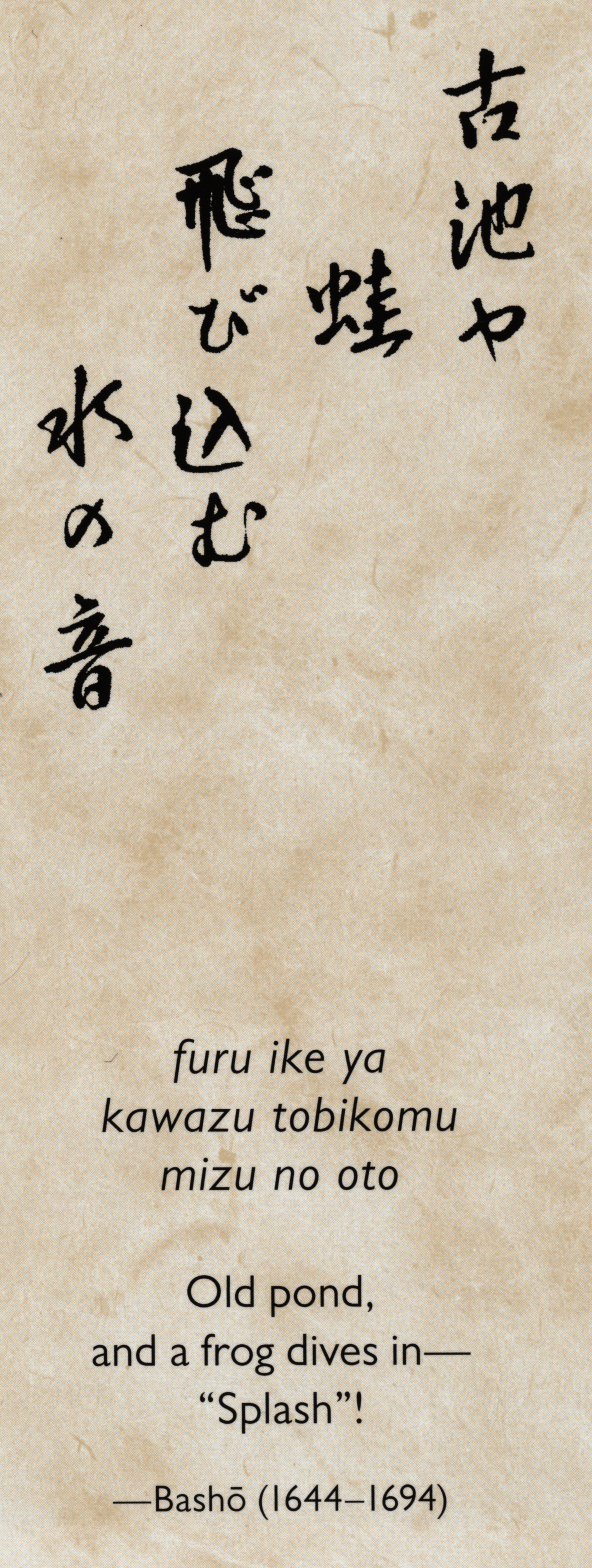
\includegraphics[width=250pt,]{Images/basho_furu_ike_ya.png}
\caption{Taken from p.42 of \textit{Haiku: Japanese Art and Poetry}. Judith Patt, Michiko Warkentyne (calligraphy) and Barry Till. 2010.}\end{figure}
\par
\par
We might encode this as follows: \par\bgroup\index{div=<div>|exampleindex}\index{lg=<lg>|exampleindex}\index{style=@style!<lg>|exampleindex}\index{l=<l>|exampleindex}\index{l=<l>|exampleindex}\index{l=<l>|exampleindex}\index{l=<l>|exampleindex}\index{lg=<lg>|exampleindex}\index{style=@style!<lg>|exampleindex}\index{l=<l>|exampleindex}\index{l=<l>|exampleindex}\index{l=<l>|exampleindex}\index{lg=<lg>|exampleindex}\index{l=<l>|exampleindex}\index{l=<l>|exampleindex}\index{l=<l>|exampleindex}\exampleFont \begin{shaded}\noindent\mbox{}{<\textbf{div}>}\mbox{}\newline 
\hspace*{1em}{<\textbf{lg}\hspace*{1em}{xml:lang}="{ja}"\mbox{}\newline 
\hspace*{1em}\hspace*{1em}{style}="{writing-mode: vertical-rl}">}\mbox{}\newline 
\hspace*{1em}\hspace*{1em}{<\textbf{l}>}{\textJapanese 古池や}{</\textbf{l}>}\mbox{}\newline 
\hspace*{1em}\hspace*{1em}{<\textbf{l}>}{\textJapanese 蛙}{</\textbf{l}>}\mbox{}\newline 
\hspace*{1em}\hspace*{1em}{<\textbf{l}>}{\textJapanese 飛び込む}{</\textbf{l}>}\mbox{}\newline 
\hspace*{1em}\hspace*{1em}{<\textbf{l}>}{\textJapanese 水の音}{</\textbf{l}>}\mbox{}\newline 
\hspace*{1em}{</\textbf{lg}>}\mbox{}\newline 
\hspace*{1em}{<\textbf{lg}\hspace*{1em}{xml:lang}="{ja-Latn}"\mbox{}\newline 
\hspace*{1em}\hspace*{1em}{style}="{writing-mode: horizontal-tb}">}\mbox{}\newline 
\hspace*{1em}\hspace*{1em}{<\textbf{l}>}{\textJapanese furu ike ya}{</\textbf{l}>}\mbox{}\newline 
\hspace*{1em}\hspace*{1em}{<\textbf{l}>}{\textJapanese kawazu tobikomu}{</\textbf{l}>}\mbox{}\newline 
\hspace*{1em}\hspace*{1em}{<\textbf{l}>}{\textJapanese mizu no oto}{</\textbf{l}>}\mbox{}\newline 
\hspace*{1em}{</\textbf{lg}>}\mbox{}\newline 
\hspace*{1em}{<\textbf{lg}\hspace*{1em}{xml:lang}="{en}">}\mbox{}\newline 
\hspace*{1em}\hspace*{1em}{<\textbf{l}>}Old pond,{</\textbf{l}>}\mbox{}\newline 
\hspace*{1em}\hspace*{1em}{<\textbf{l}>}and a frog dives in—{</\textbf{l}>}\mbox{}\newline 
\hspace*{1em}\hspace*{1em}{<\textbf{l}>}"Splash"!{</\textbf{l}>}\mbox{}\newline 
\hspace*{1em}{</\textbf{lg}>}\mbox{}\newline 
{</\textbf{div}>}\end{shaded}\egroup\par \par
For the sake of simplicity, we have not attempted to capture in this encoding such aspects as the indenting of lines in the first Japanese version, or the central alignment of the other two versions, nor any other renditional features such as font weight or size etc. The Japanese transcription has \texttt{writing-mode: vertical-rl}, which is required because Japanese may be written either in this mode or horizontally. The transcription in romaji uses the attribute {\itshape xml:lang} to supply a value of ja-Latn, indicating Japanese written in Latin script. Its {\itshape style} attribute specifies a horizontal writing mode; this may seem superfluous, but vertically-written romaji is not unknown.
\subsubsection[{Vertical Text with Embedded Horizontal Text}]{Vertical Text with Embedded Horizontal Text}\label{WDWMEG2}\par
When Japanese is written vertically, the glyph orientation remains the same as when it is written horizontally. In other words, glyphs are not rotated (although as noted above some different glyphs may be used for some characters, in particular for punctuation which needs to be positioned differently in vertical and in horizontal text). However, it is very common for languages written vertically to have embedded runs of text from languages which are normally written horizontally. This raises the issue of the orientation of the glyphs from the horizontal language. Are they written upright, as they would normally appear in horizontal text runs, or are they rotated? Consider this fragment from a Japanese article about the Indonesian language, which takes the form of a glossary list: \par
\begin{figure}[htbp]
\noindent\noindent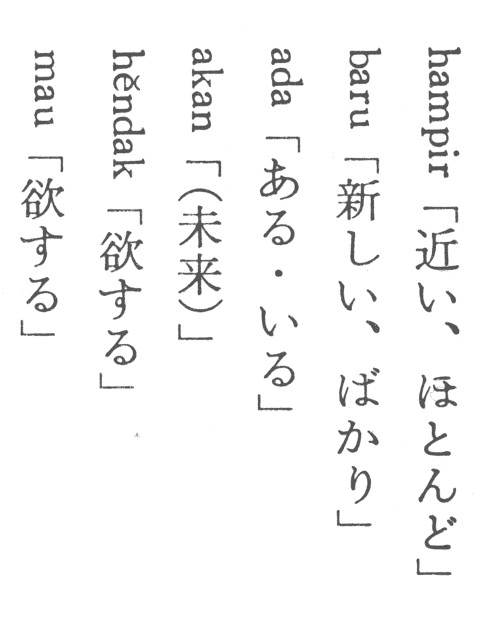
\includegraphics[width=500pt,height=624pt,]{Images/ja_vertical_indonesian_frag.jpg}
\caption{Detail from p.62 of \textit{インドネシア語". 崎山理. 1985. 外国語との対照 II. 講座日本語学 11.}}\end{figure}
\par
The text-orientation property allows us to indicate whether or not glyphs are rotated. In the following example, we have indicated that the list uses a \texttt{vertical-rl} writing mode, but that the orientation of individual glyphs may vary:\par\bgroup\index{list=<list>|exampleindex}\index{type=@type!<list>|exampleindex}\index{style=@style!<list>|exampleindex}\index{label=<label>|exampleindex}\index{item=<item>|exampleindex}\index{label=<label>|exampleindex}\index{item=<item>|exampleindex}\exampleFont \begin{shaded}\noindent\mbox{}{<\textbf{list}\hspace*{1em}{type}="{gloss}"\hspace*{1em}{xml:lang}="{ja}"\mbox{}\newline 
\hspace*{1em}{style}="{writing-mode: vertical-rl; text-orientation: mixed}">}\mbox{}\newline 
\hspace*{1em}{<\textbf{label}\hspace*{1em}{xml:lang}="{id}">}hampir{</\textbf{label}>}\mbox{}\newline 
\hspace*{1em}{<\textbf{item}>}{\textJapanese 「近い、ほとんど」}{</\textbf{item}>}\mbox{}\newline 
\hspace*{1em}{<\textbf{label}\hspace*{1em}{xml:lang}="{id}">}baru{</\textbf{label}>}\mbox{}\newline 
\hspace*{1em}{<\textbf{item}>}{\textJapanese 「新しい、ばかい」}{</\textbf{item}>}\mbox{}\newline 
\textit{<!--{\textJapanese  ... }-->}\mbox{}\newline 
{</\textbf{list}>}\end{shaded}\egroup\par \par
The rule \texttt{text-orientation: mixed} specifies that ‘characters from horizontal-only scripts are set sideways, i.e. 90° clockwise from their standard orientation in horizontal text. Characters from vertical scripts are set with their intrinsic orientation’ (\xref{http://www.w3.org/TR/css-writing-modes-3/\#text-orientation}{fantasai 2014}). Since the default value for \texttt{text-orientation} is \texttt{mixed}, this rule is not strictly required. However, if the Indonesian glyphs (which are roman characters) had been set vertically, like this:\par
\begin{figure}[htbp]
\noindent\noindent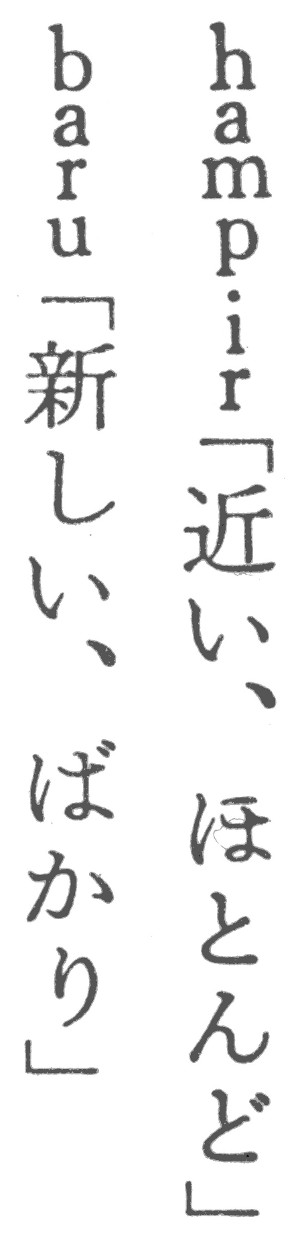
\includegraphics[width=150pt,]{Images/ja_vertical_indonesian_frag_rotated.jpg}
\caption{Fragment of previous image with Indonesian glyphs upright.}\end{figure}
\par
then an encoding like the following could be used to make this explicit: \par\bgroup\index{list=<list>|exampleindex}\index{type=@type!<list>|exampleindex}\index{style=@style!<list>|exampleindex}\index{label=<label>|exampleindex}\index{item=<item>|exampleindex}\index{label=<label>|exampleindex}\index{item=<item>|exampleindex}\exampleFont \begin{shaded}\noindent\mbox{}{<\textbf{list}\hspace*{1em}{type}="{gloss}"\hspace*{1em}{xml:lang}="{ja}"\mbox{}\newline 
\hspace*{1em}{style}="{writing-mode: vertical-rl; text-orientation: upright}">}\mbox{}\newline 
\hspace*{1em}{<\textbf{label}\hspace*{1em}{xml:lang}="{id}">}hampir{</\textbf{label}>}\mbox{}\newline 
\hspace*{1em}{<\textbf{item}>}{\textJapanese 「近い、ほとんど」}{</\textbf{item}>}\mbox{}\newline 
\hspace*{1em}{<\textbf{label}\hspace*{1em}{xml:lang}="{id}">}baru{</\textbf{label}>}\mbox{}\newline 
\hspace*{1em}{<\textbf{item}>}{\textJapanese 「新しい、ばかい」}{</\textbf{item}>}\mbox{}\newline 
\textit{<!--{\textJapanese  ... }-->}\mbox{}\newline 
{</\textbf{list}>}\end{shaded}\egroup\par \par
The rule \texttt{text-orientation: upright} specifies that ‘characters from horizontal-only scripts are rendered upright, i.e. in their standard horizontal orientation. Characters from vertical scripts are set with their intrinsic orientation and shaped normally’ (\xref{http://www.w3.org/TR/css-writing-modes-3/\#text-orientation}{fantasai 2014}).
\subsubsection[{Vertical Orientation in Horizontal Scripts}]{Vertical Orientation in Horizontal Scripts}\label{WDWMEG3}\par
It is not unusual to see text from horizontal languages written vertically even where no vertically-written script is involved. This example is a fragment from a table of information about agricultural development on Vancouver Island, written in 1855: \par
\begin{figure}[htbp]
\noindent\noindent\includegraphics[width=450pt,]{Images/bcgenesis_co_305_06_00131v_table_extract.jpg}
\caption{Enclosure with \textit{Despatch to London} 10048, CO 305/6, p. 131v from \url{https://bcgenesis.uvic.ca/V55116.html}}\end{figure}
\par
Four of the subheading cells in this fragment contain English text written vertically, bottom-to-top, to conserve space on the page. To describe this sort of phenomenon, we can use the \texttt{text-orientation} property again:\par
\texttt{text-orientation: mixed | upright | sideways-right | sideways-left | sideways | use-glyph-orientation}\par
For full details on this property, we refer the reader to the CSS Writing Modes specification. For the present example, we will make use only of the ‘sideways-left’ value, which ‘causes text to be set as if in a horizontal layout, but rotated 90° counter-clockwise.’ We might encode the third of the four cells containing vertical text like this:\par\bgroup\index{cell=<cell>|exampleindex}\index{style=@style!<cell>|exampleindex}\index{lb=<lb>|exampleindex}\index{lb=<lb>|exampleindex}\index{lb=<lb>|exampleindex}\exampleFont \begin{shaded}\noindent\mbox{}{<\textbf{cell}\hspace*{1em}{style}="{writing-mode: vertical-lr; text-orientation: sideways-left}">}\mbox{}\newline 
\hspace*{1em}{<\textbf{lb}/>}Cash Value\mbox{}\newline 
{<\textbf{lb}/>}of\mbox{}\newline 
{<\textbf{lb}/>}Farms\mbox{}\newline 
\mbox{}\newline 
{</\textbf{cell}>}\end{shaded}\egroup\par \par
The \texttt{writing-mode} property captures the fact that the script is written vertically, and its lines are to be read from left to right (so the line containing ‘of’ is to the right of that containing ‘Cash value’), while the \texttt{text-orientation} value encodes the orientation (rotated 90° counter-clockwise). We might also add \texttt{text-align: center} to the style, to express the fact that the text is centrally-aligned.
\subsubsection[{Bottom-to-top Writing}]{Bottom-to-top Writing}\label{WDWMEG4}\par
Of the rather small number of scripts which appear to be written bottom-to-top, perhaps the best-known is Ogham, an alphabet used mainly to write Archaic Irish. Ogham is typically found inscribed along the edge of a standing stone, starting at its base. The CSS Writing Modes specification does not explicitly distinguish between vertical scripts which are written top-to-bottom and those which are written bottom-to-top. Instead, such bottom-to-top scripts are best treated as left-to-right horizontal scripts, oriented vertically because of the constraints of the medium on which they are inscribed. Such scripts are analogous to the vertical English text-runs in the table cells in the example above, and can be handled in exactly the same manner (\texttt{writing-mode: vertical-lr; text-orientation: sideways-left}). In cases where writing follows a curved path (such as Ogham running around the edge of a stone), a meticulous encoder might resort to the use of SVG to describe the path, rather than treating the phenomenon as a writing mode.
\subsubsection[{Mixed Horizontal Directionality}]{Mixed Horizontal Directionality}\label{WDWMEG5}\par
Returning to our previous simple example \par\hfill\bgroup\exampleFont\vskip 10pt\begin{shaded}
\obeyspaces The Arabic term قلم رصاص means "pencil".\end{shaded}
\par\egroup 
\par
we could use the direction property to make directionality explicit:\par
\texttt{direction: ltr | rtl}\par\bgroup\index{s=<s>|exampleindex}\index{style=@style!<s>|exampleindex}\index{term=<term>|exampleindex}\index{style=@style!<term>|exampleindex}\exampleFont \begin{shaded}\noindent\mbox{}{<\textbf{s}\hspace*{1em}{xml:lang}="{en}"\hspace*{1em}{style}="{direction: ltr}">}The Arabic term\mbox{}\newline 
{<\textbf{term}\hspace*{1em}{xml:lang}="{ar}"\mbox{}\newline 
\hspace*{1em}\hspace*{1em}{style}="{direction: rtl; unicode-bidi: embed}">}\hbox{قلم رصاص}{</\textbf{term}>} means "pencil".{</\textbf{s}>}\end{shaded}\egroup\par \par
The use of the \texttt{direction} property to record the observed directionality of the text is unambiguous, even though it is (as we noted above) superfluous. The use of the \texttt{unicode-bidi} property here may require some explanation. By default this property has the value ‘normal’, the effect of which in this context would be to ignore any value supplied for the direction property. The CSS Writing Modes specification stipulates that the direction property ‘has no effect on bidi reordering when specified on inline boxes whose \texttt{unicode-bidi} property’s value is ‘normal’, because the element does not open an additional level of embedding with respect to the bidirectional algorithm.’\par
Mixed horizontal directionality is very common in languages such as Arabic and Hebrew, particularly when numbers (which are always given LTR) or phrases from LTR languages are embedded. It is not impossible, though quite unusual, for ambiguities to arise in such situations, which may give rise to the parts of a document being displayed in unexpected ways that do not correspond to the natural reading order. A more detailed discussion of this issue from an HTML perspective is provided by a W3C Internationalization Working Group report \xref{http://www.w3.org/International/articles/inline-bidi-markup/\#where}{Inline markup and bidirectional text in HTML}.
\subsubsection[{Summary}]{Summary}\par
For most texts, information about text directionality need not be explicitly encoded in a TEI text, either because it follows unambiguously from {\itshape xml:lang} values, or because it can be expected to be handled unequivocally by the Unicode Bidi Algorithm. Where it is considered important to encode such information, properties and values taken from the CSS Writing Modes module may be used by means of the global TEI {\itshape style} attribute (or using the TEI \hyperref[TEI.rendition]{<rendition>} element, linked with the {\itshape rendition} attribute). Most phenomena can be well described in this way; of those which cannot, other approaches based on the CSS Transforms module are presented in the next section.
\subsection[{Text Rotation}]{Text Rotation}\label{WDWMTT}\par
In what follows, we examine a range of textual phenomena which in some ways appear very similar to those examined above, and even overlap with them. We can categorize these as text transformation features, and suggest some strategies for encoding them based on the properties detailed in the \hyperref[CSSTM]{CSS Transforms (Fraser et al 2013)} specification. This CSS module provides a complex array of properties, values and functions which can be used to rotate, skew, translate and otherwise transform textual and graphical objects. We can borrow this vocabulary in order to describe textual phenomena in a precise manner.\par
We begin with a simple example of a rotational transform: \par
\begin{figure}[htbp]
\noindent\noindent\includegraphics[]{Images/rotation_on_z_axis.png}\end{figure}
\par
Here a block of text has been rotated around its z-axis. This is clearly not a ‘writing mode’; the writing mode for this text is horizontal, left to right. Furthermore, even if we wished to treat this as a writing mode, we could not do so, because there is no way to use writing modes properties to describe an text orientation which is angled at 45 degrees; no human languages are consistently written in this orientation. It is more appropriate to treat this as a rotational transformation. We can do this using two properties: \texttt{transform} and \texttt{transform-origin}. (Both of these properties have quite complex value sets, and we will not look at all of them here. See the \hyperref[CSSTM]{specification} for full details.)\par
The \texttt{transform} property takes as its value one or more of the transform functions, one of which is the function \texttt{rotateZ()}:\par\bgroup\index{ab=<ab>|exampleindex}\index{style=@style!<ab>|exampleindex}\exampleFont \begin{shaded}\noindent\mbox{}{<\textbf{ab}\hspace*{1em}{style}="{transform:rotateZ(-45deg)}">}TEI-C.ORG{</\textbf{ab}>}\end{shaded}\egroup\par \par
Any rotation must take place clockwise around an axis positioned relative to the element being rotated, and the \texttt{transform-origin} property can be used to specify the pivot point. By default, the value of \texttt{transform-origin} is ‘50\% 50\%’, the point at the centre of the element, but these values can be changed to reflect rotation around a different origin point. (The TEI \hyperref[TEI.zone]{<zone>} element also bears an attribute {\itshape rotate} which can specify rotation in degrees around the z-axis, but it is not available for any other element.)\par
A block of text may also be rotated about either of its other axes. For example, this shows rotation around the Y (vertical) axis: \par
\begin{figure}[htbp]
\noindent\noindent\includegraphics[]{Images/rotation_on_y_axis.png}\end{figure}
\par\bgroup\index{ab=<ab>|exampleindex}\index{style=@style!<ab>|exampleindex}\exampleFont \begin{shaded}\noindent\mbox{}{<\textbf{ab}\hspace*{1em}{style}="{transform:rotateY(45deg)}">}TEI-C.ORG{</\textbf{ab}>}\end{shaded}\egroup\par \par
These are obviously trivial examples, but similar features do appear in historical texts. George Herbert's \textit{The Temple} includes two stanzas headed ‘Easter Wings’ which are both normally printed in a rotated form so that they represent a pair of wings:\par
\begin{figure}[htbp]
\noindent\noindent\includegraphics[width=300pt,]{Images/herbert_church_p35_sm.jpg}
\caption{Page 35 of George Herbert's \textit{The Temple} (1633), from a copy in the Folger Library.}\end{figure}
\par
This could be encoded thus: \par\bgroup\index{lg=<lg>|exampleindex}\index{style=@style!<lg>|exampleindex}\index{l=<l>|exampleindex}\index{l=<l>|exampleindex}\exampleFont \begin{shaded}\noindent\mbox{}{<\textbf{lg}\hspace*{1em}{style}="{transform:rotateZ(90deg)}">}\mbox{}\newline 
\hspace*{1em}{<\textbf{l}>}My tender age in ſorrow did beginne:{</\textbf{l}>}\mbox{}\newline 
\hspace*{1em}{<\textbf{l}>}And ſtill with ſickneſſes and ſhame{</\textbf{l}>}\mbox{}\newline 
\textit{<!-- ... -->}\mbox{}\newline 
{</\textbf{lg}>}\end{shaded}\egroup\par \par
We might also argue that this is in fact a vertical writing mode by supplying \texttt{writing-mode: vertical-rl; text-orientation: sideways-right} as the value for the {\itshape style} attribute in the preceding example.\par
Rotation is also useful as a method of handling a true writing mode which is not covered by the CSS Writing Modes: \textit{boustrophedon}. This is a writing mode common in inscriptions in Latin, Greek and other languages, in which alternate lines run from left to right and from right to left\footnote{The name is taken from the Greek βουστροφηδόν, meaning ‘ox-turning’ from βοῦς (an ox) and στροφή (‘turn’); that is, turning as an ox does when pulling a plough.}. Right-to-left lines in boustrophedon have another unexpected feature: their glyphs are reversed, so that these lines appear as ‘mirror writing’, as in the following ancient Greek inscription: \begin{figure}[htbp]
\noindent\noindent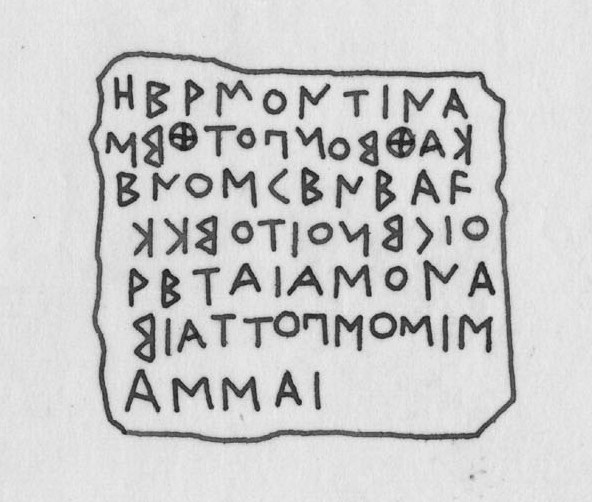
\includegraphics[width=592pt,height=502pt,]{Images/boustrophedon_small_J_NW_Epeiros_13_p03.jpg}
\caption{Leaden plaque bearing an inquiry by Hermon from the oracular precinct at Dodona. (L.H. Jeffery Archive)}\end{figure}
\par
This might be transcribed as follows (ignoring word boundaries for the moment): \par\bgroup\index{ab=<ab>|exampleindex}\index{lb=<lb>|exampleindex}\index{lb=<lb>|exampleindex}\index{seg=<seg>|exampleindex}\index{style=@style!<seg>|exampleindex}\index{lb=<lb>|exampleindex}\index{lb=<lb>|exampleindex}\index{seg=<seg>|exampleindex}\index{style=@style!<seg>|exampleindex}\index{lb=<lb>|exampleindex}\index{lb=<lb>|exampleindex}\index{seg=<seg>|exampleindex}\index{style=@style!<seg>|exampleindex}\index{lb=<lb>|exampleindex}\exampleFont \begin{shaded}\noindent\mbox{}{<\textbf{ab}>}\mbox{}\newline 
\hspace*{1em}{<\textbf{lb}/>}ΗΕΡΜΟΝΤΙΝA\mbox{}\newline 
{<\textbf{lb}/>}\mbox{}\newline 
\hspace*{1em}{<\textbf{seg}\hspace*{1em}{style}="{rotateY(180deg)}">}ΚΑΘΕΟΝΠΟΤΘΕΜ{</\textbf{seg}>}\mbox{}\newline 
\hspace*{1em}{<\textbf{lb}/>}ΕΝΟΣΥΕΝΕΑϜ\mbox{}\newline 
{<\textbf{lb}/>}\mbox{}\newline 
\hspace*{1em}{<\textbf{seg}\hspace*{1em}{style}="{rotateY(180deg)}">}ΟΙΥΕΝΟΙΤΙΕΚΚ{</\textbf{seg}>}\mbox{}\newline 
\hspace*{1em}{<\textbf{lb}/>}ΡΕΤΑΙΑΣΟΝΑ\mbox{}\newline 
{<\textbf{lb}/>}\mbox{}\newline 
\hspace*{1em}{<\textbf{seg}\hspace*{1em}{style}="{rotateY(180deg)}">}ΣΙΜΟΣΟΤΤΑΙΕ{</\textbf{seg}>}\mbox{}\newline 
\hspace*{1em}{<\textbf{lb}/>}ΑΣΣΑΙ\mbox{}\newline 
\mbox{}\newline 
{</\textbf{ab}>}\end{shaded}\egroup\par \par
The 180-degree rotation around the Y (vertical) axis here describes what is happening in the RTL line in boustrophedon; the order of glyphs is reversed, and so is their individual orientation (in fact, we see them ‘from the back’, as it were). \hyperref[TEI.seg]{<seg>} elements have been used here because these are clearly not ‘lines’ in the sense of poetic lines; the text is continuous prose, and linebreaks are incidental.\par
There are obviously some unsatisfactory aspects of this manner of encoding boustrophedon. In the inscription above, some words run across linebreaks, so if we wished to tag both words and the right-to-left phenomena, one hierarchy would have to be privileged over the other. By using a transform function rather than a writing mode property, we are apparently suggesting that boustrophedon is not in fact a writing mode, whereas it clearly is. But the CSS Writing Modes specification does not provide support for boustrophedon, because it is a rather obscure historical phenomenon; using a rotational transform is one practical alternative. 
\subsection[{Caveat}]{Caveat}\label{WDCAV}\par
As with other parts of the CSS specification, the intended effect of CSS Transforms properties and values is defined with reference to a specific \xref{http://www.w3.org/TR/CSS2/visuren.html}{Visual formatting model}; the language is designed to describe how an HTML document should be formatted. This is not, of course, the case for the TEI, which lacks any explicit processing or formatting model, and attempts to define objects as far as possible without consideration of their visual appearance. As long as the properties and values from the CSS Transforms module are used as a convenient, well-specified descriptive language to capture features of a text, without any expectation of using them directly and reliably for rendering, this is not particularly problematic. CSS provides a useful and well-defined vocabulary to describe many aspects of the appearance of source texts, benefitting particularly from the clarity of definition provided by the specification. However, if there is any expectation of using this information to render a text in a predictable and accurate way, it will be essential to provide enough styling information throughout the document hierarchy to resolve all ambiguities with regard to size, positioning, block status, etc. before any element undergoes a transform operation.
\subsection[{Formal Definition}]{Formal Definition}\label{WSD-DEF}\par
The gaiji module described in this chapter makes available the following components: \begin{description}

\item[{Module gaiji: Character and glyph documentation}]\hspace{1em}\hfill\linebreak
\mbox{}\\[-10pt] \begin{itemize}
\item {\itshape Elements defined}: \hyperref[TEI.char]{char} \hyperref[TEI.charDecl]{charDecl} \hyperref[TEI.charName]{charName} \hyperref[TEI.charProp]{charProp} \hyperref[TEI.g]{g} \hyperref[TEI.glyph]{glyph} \hyperref[TEI.glyphName]{glyphName} \hyperref[TEI.localName]{localName} \hyperref[TEI.localProp]{localProp} \hyperref[TEI.mapping]{mapping} \hyperref[TEI.unicodeName]{unicodeName} \hyperref[TEI.unicodeProp]{unicodeProp} \hyperref[TEI.unihanProp]{unihanProp} \hyperref[TEI.value]{value}
\item {\itshape Classes defined}: \hyperref[TEI.att.gaijiProp]{att.gaijiProp}
\end{itemize} 
\end{description}  The selection and combination of modules to form a TEI schema is described in \textit{\hyperref[STIN]{1.2.\ Defining a TEI Schema}}.